El algoritmo de rosenbrock se basa en el proceso de ortonormalización de Gram-Schmidt para generar una base ortonormal. Tras esto, se optimiza en dichas direcciones, generando una series de puntos que después se usaran para construir otra base ortonormal y repetir el proceso.

Entre los problemas que se nos plantearon con el alg. lineal estaba el del punto iniciale y el $\epsilon$ a usar. Para resolver el primero tomamos el punto a partir del cual restringíamos con un tamaño de paso (de 1000 a 100000). Para el problema del $\epsilon$ de parada, sencillamente pasamos el que usamos en el algoritmo. El criterio estándar seguido es: $|| f(x_k) - f(x_{k+1}) || < \epsilon$  o $|| f(x_{k+1} ||< \epsilon$
% \begin{displaymath}
%   \begin{array}{l@{ \hspace{3ex}\textrm{ o }\hspace{3ex} }r} 
%     || f(x_k) - f(x_{k+1}) || < \epsilon & || f(x_{k+1} < \epsilon || \\ \end{array}
% \end{displaymath}


Estos son algunos resultado usando el algoritmo de la sección áurea como algoritmo de optimización lineal:
\begin{table}[H]
\hfill\begin{tabular}{|c|cccccc|c|} \hline
\bf point  & \bf eps & \bf maxit & \bf path & \bf eval & \bf diff    & \bf final           & \bf function                \\\hline\hline
(0,0)      & 0.0005  & 10000     & 10000    & 1360002  & -81.1848    & (-8.06544,65.0564)  & \multirow{4}{*}{Rosenbrock} \\
(10,-10)   & 0.0005  & 10000     & 10000    & 1360002  & 1.20956e+06 & (-21.7229,471.89)   &                             \\
(0,10)     & 0.0005  & 10000     & 10000    & 1360002  & 9272.37     & (27.9931,783.614)   &                             \\
(-1,1)     & 0.0005  & 10000     & 2        & 274      & 4           & (0.999968,0.99994)  &                             \\\hline\hline
(0.001,10) & 0.0005  & 10000     & 7        & 954      & 10.2313     & (-122.76,-0.71873)  & \multirow{3}{*}{Patata}     \\
(10,10)    & 0.0005  & 10000     & 10000    & 1360002  & 10.2107     & (833.428,-0.85336)  &                             \\
(10,0)     & 0.0005  & 10000     & 10000    & 1360002  & 0.23134     & (49.5971,0.0256535) &                             \\\hline
\end{tabular}\hfill\hbox{}
\caption{Resultados del algoritmo de Rosenbrock}
\end{table}
\vspace{-1em}

\begin{wrapfigure}{r}{0.6\textwidth}
\vspace{-8.6em}\hfill%
\hspace{-6ex}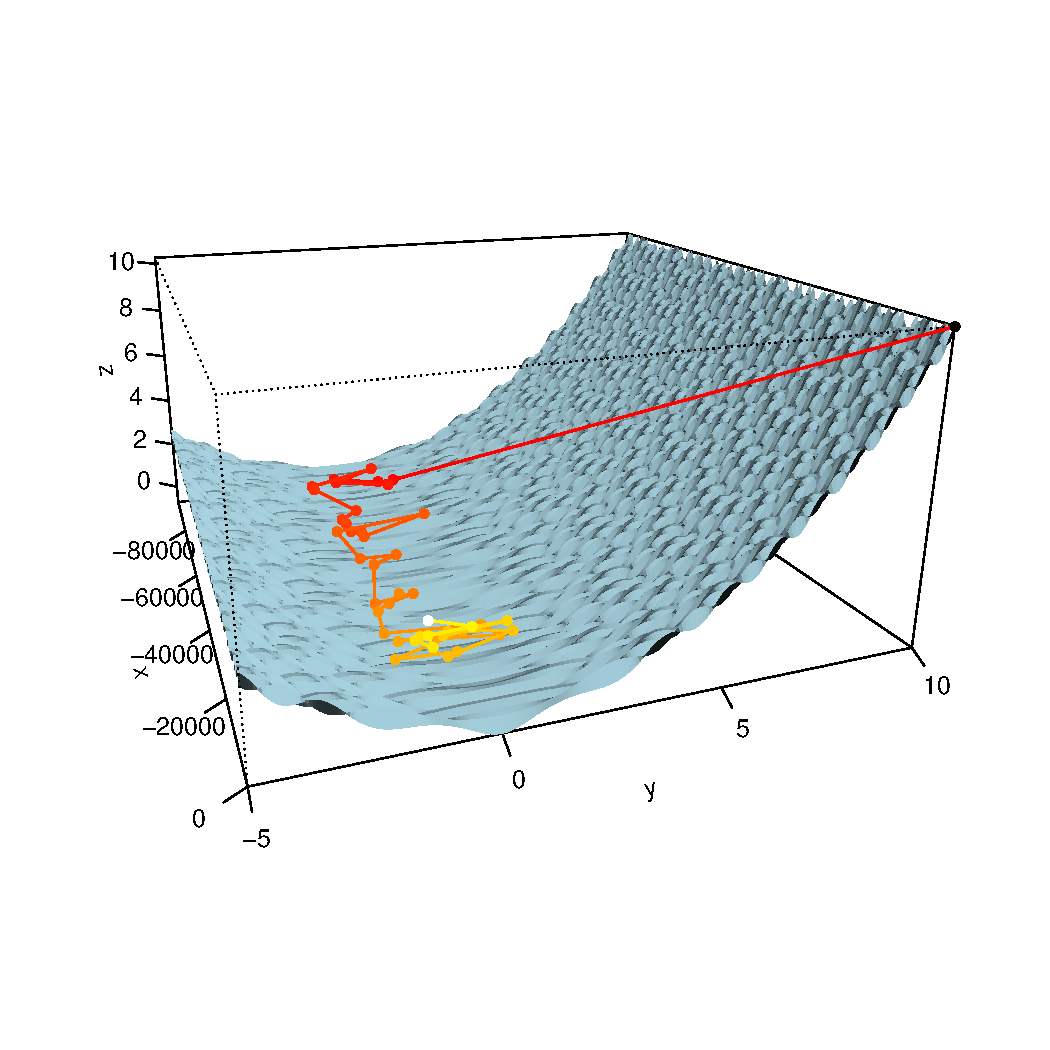
\includegraphics[width=1.2\linewidth]{../theoretic_study/func_patata/R/0,10/plot3.pdf}%
\hfill\hbox{}
\vspace{-8em}
\caption{\small función patata y sec. aurea con paso de 100000, $x_0=(0,10)$} \label{fig:rosen1}
\vspace{-5em}
\end{wrapfigure}
Como se puede ver por los resultados, a pesar que el algoritmo comience en un punto relativamente cercano a un mínimo global, tiende a alejarse considerablemente de éste, siendo la mayoría de los puntos finales alejados del origen. La \hyperref[fig:rosen1]{Figura \ref*{fig:rosen1}} en la que el algoritmo se aleja del mínimo global $(0,0)$ en la primera iteración, es un ejemplo claro de esto.

La razón de esto es que el algoritmo carece de información del entorno del punto, tan solo conoce la información obtenida al mejorar iterativamente por las rectas, dando casos muy malos como el del primer punto, en el cual se llega incluso a empeorar. 
\newpage
% Esto podría deberse al algoritmo de optimización lineal que hemos implementado, pero por lo general la tendencia se debería mantener independientemente del algoritmo que se use.

\begin{wrapfigure}{l}{0.5\textwidth}
\vspace{-4em}\hfill%
\hspace{-5ex}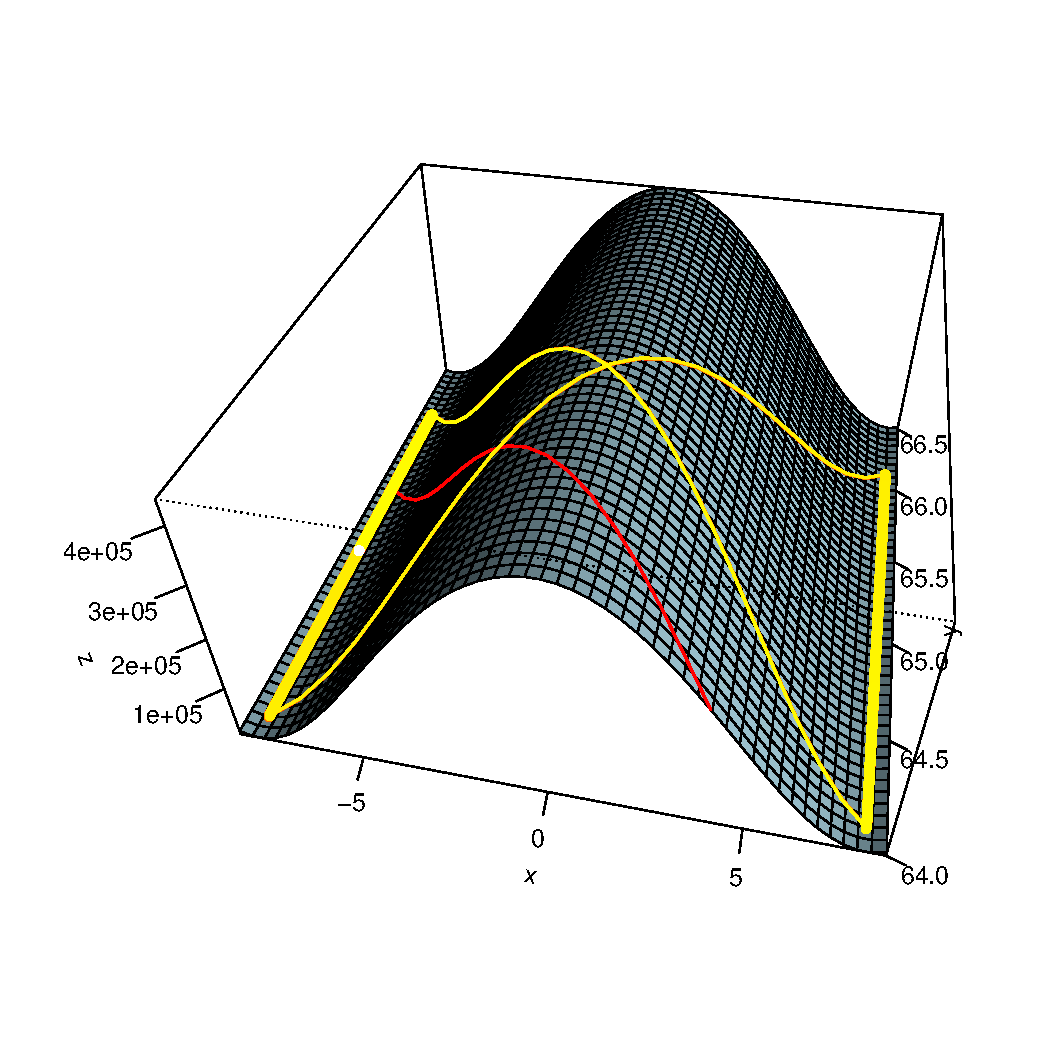
\includegraphics[width=1\linewidth]{../graphs/rosenbrock_fun/rosen/rosen_plot3.pdf}%
\hfill\hbox{}
\vspace{-4em}
\caption{\small ciclos en la función de rosenbrock con $x_0=(0,0)$} \label{fig:rosen2}
\vspace{-4.5em}
\end{wrapfigure}

Otro caso que cabe destacar es el reflejado en la \hyperref[fig:rosen2]{Figura \ref*{fig:rosen2}}. En este caso concreto el algoritmo salta de un lado al otro del valle tras unos cientos de iteraciones, terminando cuando ha agotado su número máximo de iteraciones.

Este caso es recurrente. Los puntos que se van obteniendo están contenidos en unos ciertos intervalos que se repiten tras algunas iteraciones. Esto puede ser debido a la manera en la que se genera una nueva base a partir de la anterior por el método de Gram-Schmidt, que no es capaz de generar la sufiente ``diversidad'' de bases y éstas terminan repitiendose, generando ciclos en las soluciones.
